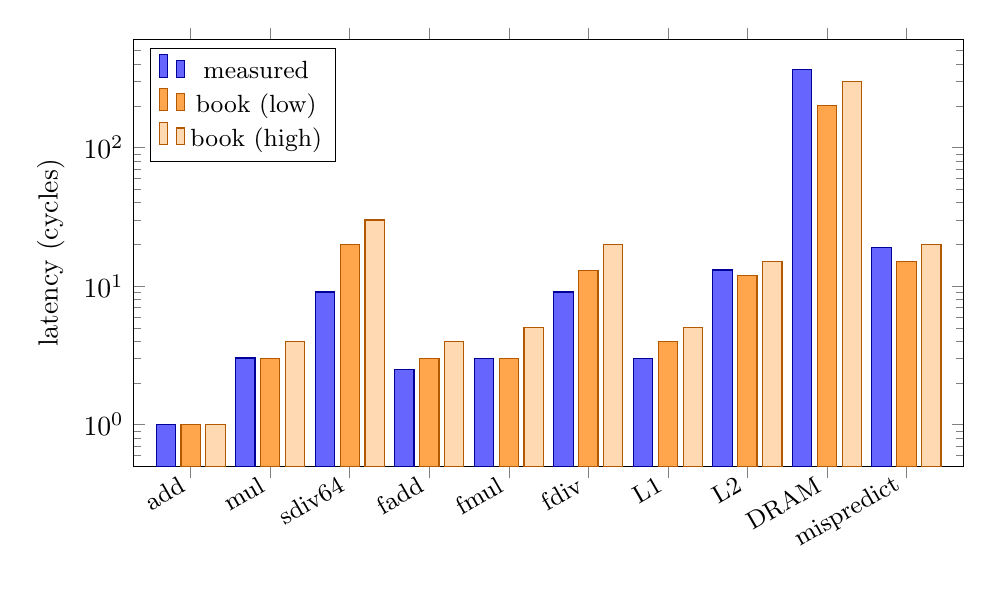
\begin{tikzpicture}
\begin{axis}[ybar, ymode=log, log origin=infty, width=\textwidth, height=7cm, bar width=7pt,
  symbolic x coords={add,mul,sdiv64,fadd,fmul,fdiv,L1,L2,DRAM,mispredict}, xtick=data,
  x tick label style={rotate=30, anchor=east, font=\small}, ylabel={latency (cycles)},
  legend style={at={(0.02,0.98)}, anchor=north west, font=\small}, ymin=0.5, ymax=600, enlarge x limits=0.08]
\addplot+[fill=blue!60, draw=blue!60!black] coordinates {(add,1.00) (mul,3.03) (sdiv64,9.06) (fadd,2.50) (fmul,3.02) (fdiv,9.06) (L1,3.02) (L2,13.08) (DRAM,365.79) (mispredict,19.01)};
\addplot+[fill=orange!70, draw=orange!70!black] coordinates {(add,1) (mul,3) (sdiv64,20) (fadd,3) (fmul,3) (fdiv,13) (L1,4) (L2,12) (DRAM,200) (mispredict,15)};
\addplot+[fill=orange!30, draw=orange!70!black] coordinates {(add,1) (mul,4) (sdiv64,30) (fadd,4) (fmul,5) (fdiv,20) (L1,5) (L2,15) (DRAM,300) (mispredict,20)};
\legend{measured, book (low), book (high)}
\end{axis}
\end{tikzpicture}